161. \begin{figure}[ht!]
\center{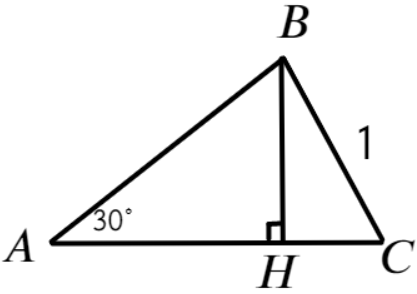
\includegraphics[scale=0.35]{g8-160.png}}
\end{figure}\\
Прямоугольный треугольник вписан в окружность, центром которой является середина его гипотенузы, а радиусом --- её половина. Медиана $AM,$ проведённая из прямого угла, равна половине гипотенузы, то есть $2:2=1.$ Проведём высоту $AH,$ тогда в треугольнике $AMH$ отрезок $AM$ является гипотенузой, значит $AH\leqslant AM=1.$ Таким образом, $S_{\Delta ABC}=\cfrac{1}{2}AH\cdot BC \leqslant \cfrac{1}{2}\cdot 1 \cdot 2=1.$ Равенство достигается в том случае, когда $AH$ совпадает с $AM,$ то есть треугольник $ABC$ является равнобедренным.\newpage\noindent
